\subsection{理論値との比較}
通常の球形粒子にbotton heavy性を仮定した場合について理論値との比較を行う.
この場合,\ref{sec:rotation}で述べたように,粒子にかかるトルクは,式\eqref{eq:sum_of_torque_z}のように表される.
    \begin{align}
        N_z &= \boldsymbol{N}^\mathrm{H}_z + \boldsymbol{N}^\mathrm{b.h.}_z \notag \\
            &= 4 \pi \mu a^3 \dot{\gamma} - \frac{4}{3} \pi \rho h g \sin \theta
        \tag{\ref{eq:sum_of_torque_z}}
    \end{align}

\noindent
このトルクはFig.\ref{fig:sum_of_torque}のように表される.

    \begin{figure}[H]
        \centering
        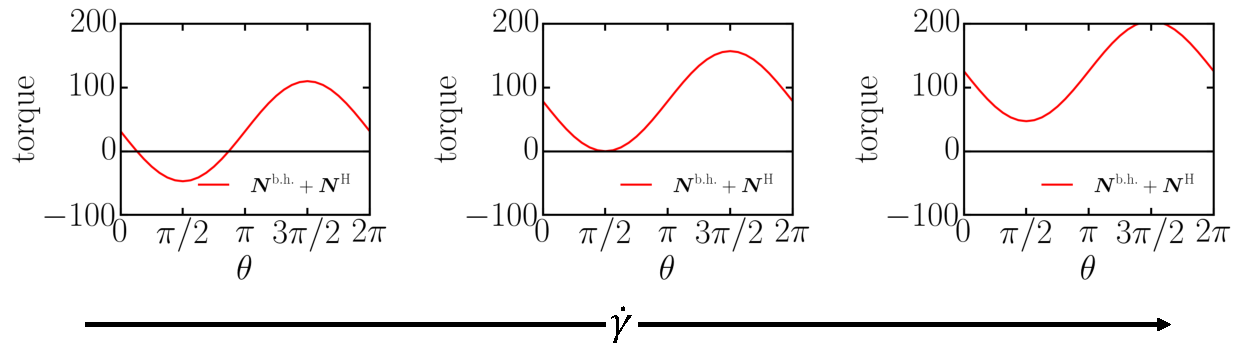
\includegraphics[scale=0.8]{/Users/taiga/Projects/lab/thesis/components/chapter4/figs/sum_of_torque.pdf}
        \caption{流体から受けるトルクとbottom heavy性によるトルクの和}
        \label{fig:sum_of_torque}
    \end{figure}

\noindent
本研究では,粒子の重心と球の中心のずれを$h = 2.5 \Delta$,重力の大きさを$g = 0.06$と設定した.
$\dot{\gamma} < 0.05$の場合には粒子の進行方向は$0 < \theta < \pi / 2$のある角度に固定され,
$\dot{\gamma} = 0.05$の場合に,粒子の進行方向は$\theta = \pi /2$に固定され,
$\dot{\gamma} > 0.05$の場合に定常的に回転すると予想される.
Fig.\ref{fig:extracted_results}は,Fig.\ref{fig:simulation_results}の上段のシミュレーション結果を抜粋したものである.

    \begin{figure}[htbp]
        \centering
        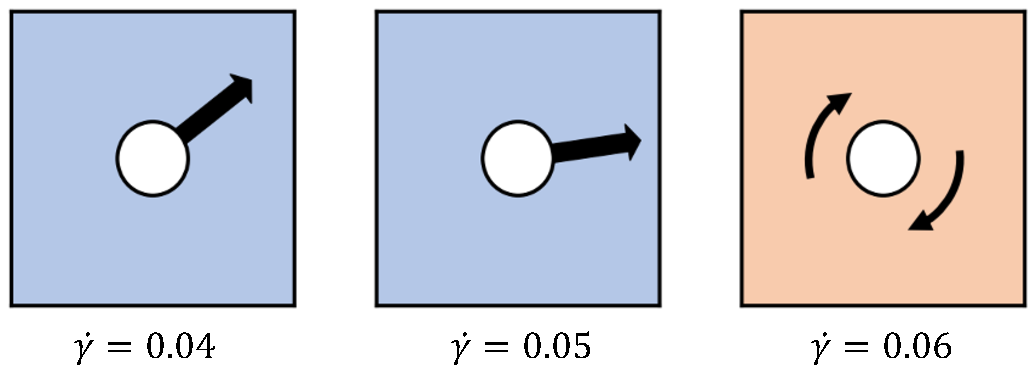
\includegraphics[scale=0.8]{/Users/taiga/Projects/lab/thesis/components/chapter4/figs/extracted_results.pdf}
        \caption{$B_2 = 0$の場合のシミュレーション模式図とそのときのせん断速度の値}
        \label{fig:extracted_results}
    \end{figure}

\noindent
この図から,シミュレーション結果が示す粒子の挙動は,理論的な式によって導かれる挙動とよく一致していることが分かる.
